\chapter{Fundamentals}
\label{sec:fundamentals}

The core topic of this thesis falls under the category of machine learning. Thus, first the concept of machine learning and the tasks related to the approach of this thesis are explained. Second, means used for evaluation of the approach are discussed.

\section{Machine Learning}
In this section, the aspects of the field of machine learning which are relevant for this thesis are going to be introduced briefly. The core of machine learning is learning algorithms, which are used to induce a general model from a set of data samples. The concept of machine learning will be explained here with the help of an example. % Further what happens exactly here 

Suppose an aspiring gardener wants to learn how to distinguish between different species of iris plants, a genus of ornamental plants with colorful flowers. More specifically, the focus lies on the three species iris versicolor, virginica and setosa. In order to do so, the gardener has observed four different \textit{features}, namely the length and width of their petals and sepals, for a number of different individuals for which he knows the species, which is illustrated in Table \ref{tab:iris}. The goal of the gardener is then to learn how to distinguish the species based on these features, that is to derive a \textit{model} from the data that will predict which species (out of the considered three) an unknown iris plant is. The gardener decides to build a decision tree from the data with forks on the basis of feature values, so that they can determine the species of the plant without much calculation. They observe that all iris setosa plants from his sample have a petal width of $\leq 0.6 $ cm, and that of the plants with a petal width of $>0.6$ cm, most plants with a petal width $\leq 1.7$ cm are of the iris versicolor species. The remaining plants with a petal width of $>1.7$ cm are mostly iris virginica plants. While this model (illustrated in Figure \ref{fig:decision_tree}) will not correctly predict the species of all iris plants, the gardener is settles with the approximation they have found.

\begin{table}[h]
	\begin{tabularx}{\textwidth}{>{\raggedleft\arraybackslash}X | >{\raggedleft\arraybackslash}X | >{\raggedleft\arraybackslash}X | >{\raggedleft\arraybackslash}X | X}
		%\hline
		\multicolumn{1}{X}{Sepal length}	& \multicolumn{1}{X}{Sepal width}	& \multicolumn{1}{X}{Petal length}	& \multicolumn{1}{X}{Petal width} & Species			\\ \hline
				5.1			& 3.5			& 1.4			& 0.2			& Iris setosa		\\ 
				5.0			& 3.5			& 1.6			& 0.6			& Iris setosa		\\ 
				5.0			& 3.4			& 1.6			& 0.4			& Iris setosa		\\ 
				5.6			& 3.0			& 4.5			& 1.5			& Iris versicolor	\\ 				
				6.7			& 3.1			& 4.4			& 1.4			& Iris versicolor	\\ 	
				5.9			& 3.2			& 4.8			& 1.8			& Iris versicolor	\\ 	
				7.2			& 3.0			& 5.8			& 1.6			& Iris virginica		\\ 	
				5.9			& 3.0			& 5.1			& 1.8			& Iris virginica		\\ 
				6.9			& 3.1			& 5.1			& 2.3			& Iris virginica		\\ 	
	\end{tabularx}
	\caption{Features of different iris plants. This is an excerpt from the well known iris data set \cite{iris}}
	\label{tab:iris}
\end{table}

%\tikzsetnextfilename{DecisionTree}
\begin{figure}
\centering
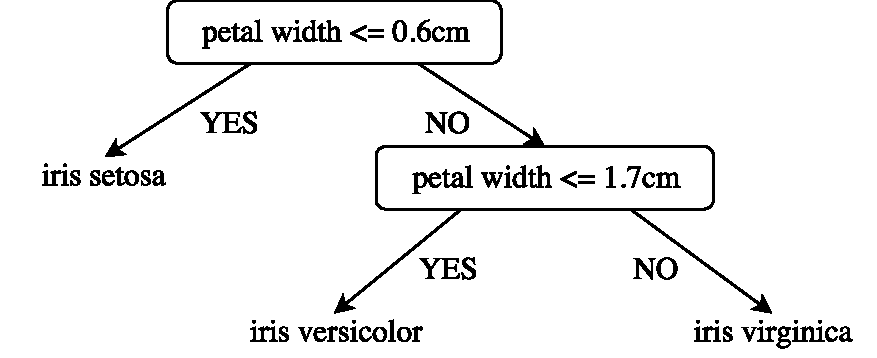
\includegraphics[scale=.75]{gfx/decision_tree.pdf}
\caption{The decision tree constructed as a simple model  to classify iris plants in the gardening example.}
\label{fig:decision_tree}
\end{figure}

In formal terms, the gardener is searching for an unknown \textit{target function} $f:X \rightarrow Y$ from the input space $X$ to the output space $Y$ \cite{abu2012learning} that represents an ideal way of identifying iris species. $X$ denotes the possible inputs, in this case all combinations of the four features that have been defined, whereas $Y$ are the outputs, here the species of iris plant. The examples that the gardener recorded are samples $(x_1,y_1),(x_2,y_2),\dots,(x_n,y_n)$ from $f$ such that $f(x_i)=y_i$. Together, they form a data set $D$ which is one of all possible data sets $\mathbb{D}$ for the problem. They then choose a specific approximation $g:X \rightarrow Y,g\approx f$, the decision tree they built, from the hypothesis space $H$, which in this case consists of possible decision trees. The learning algorithm itself thus maps a data set to a hypothesis from the hypothesis space and can be defined as $A:\mathbb{D}\rightarrow H$. An overview of this learning problem is provided in Figure \ref{fig:learning_problem}.

\begin{figure}
\centering
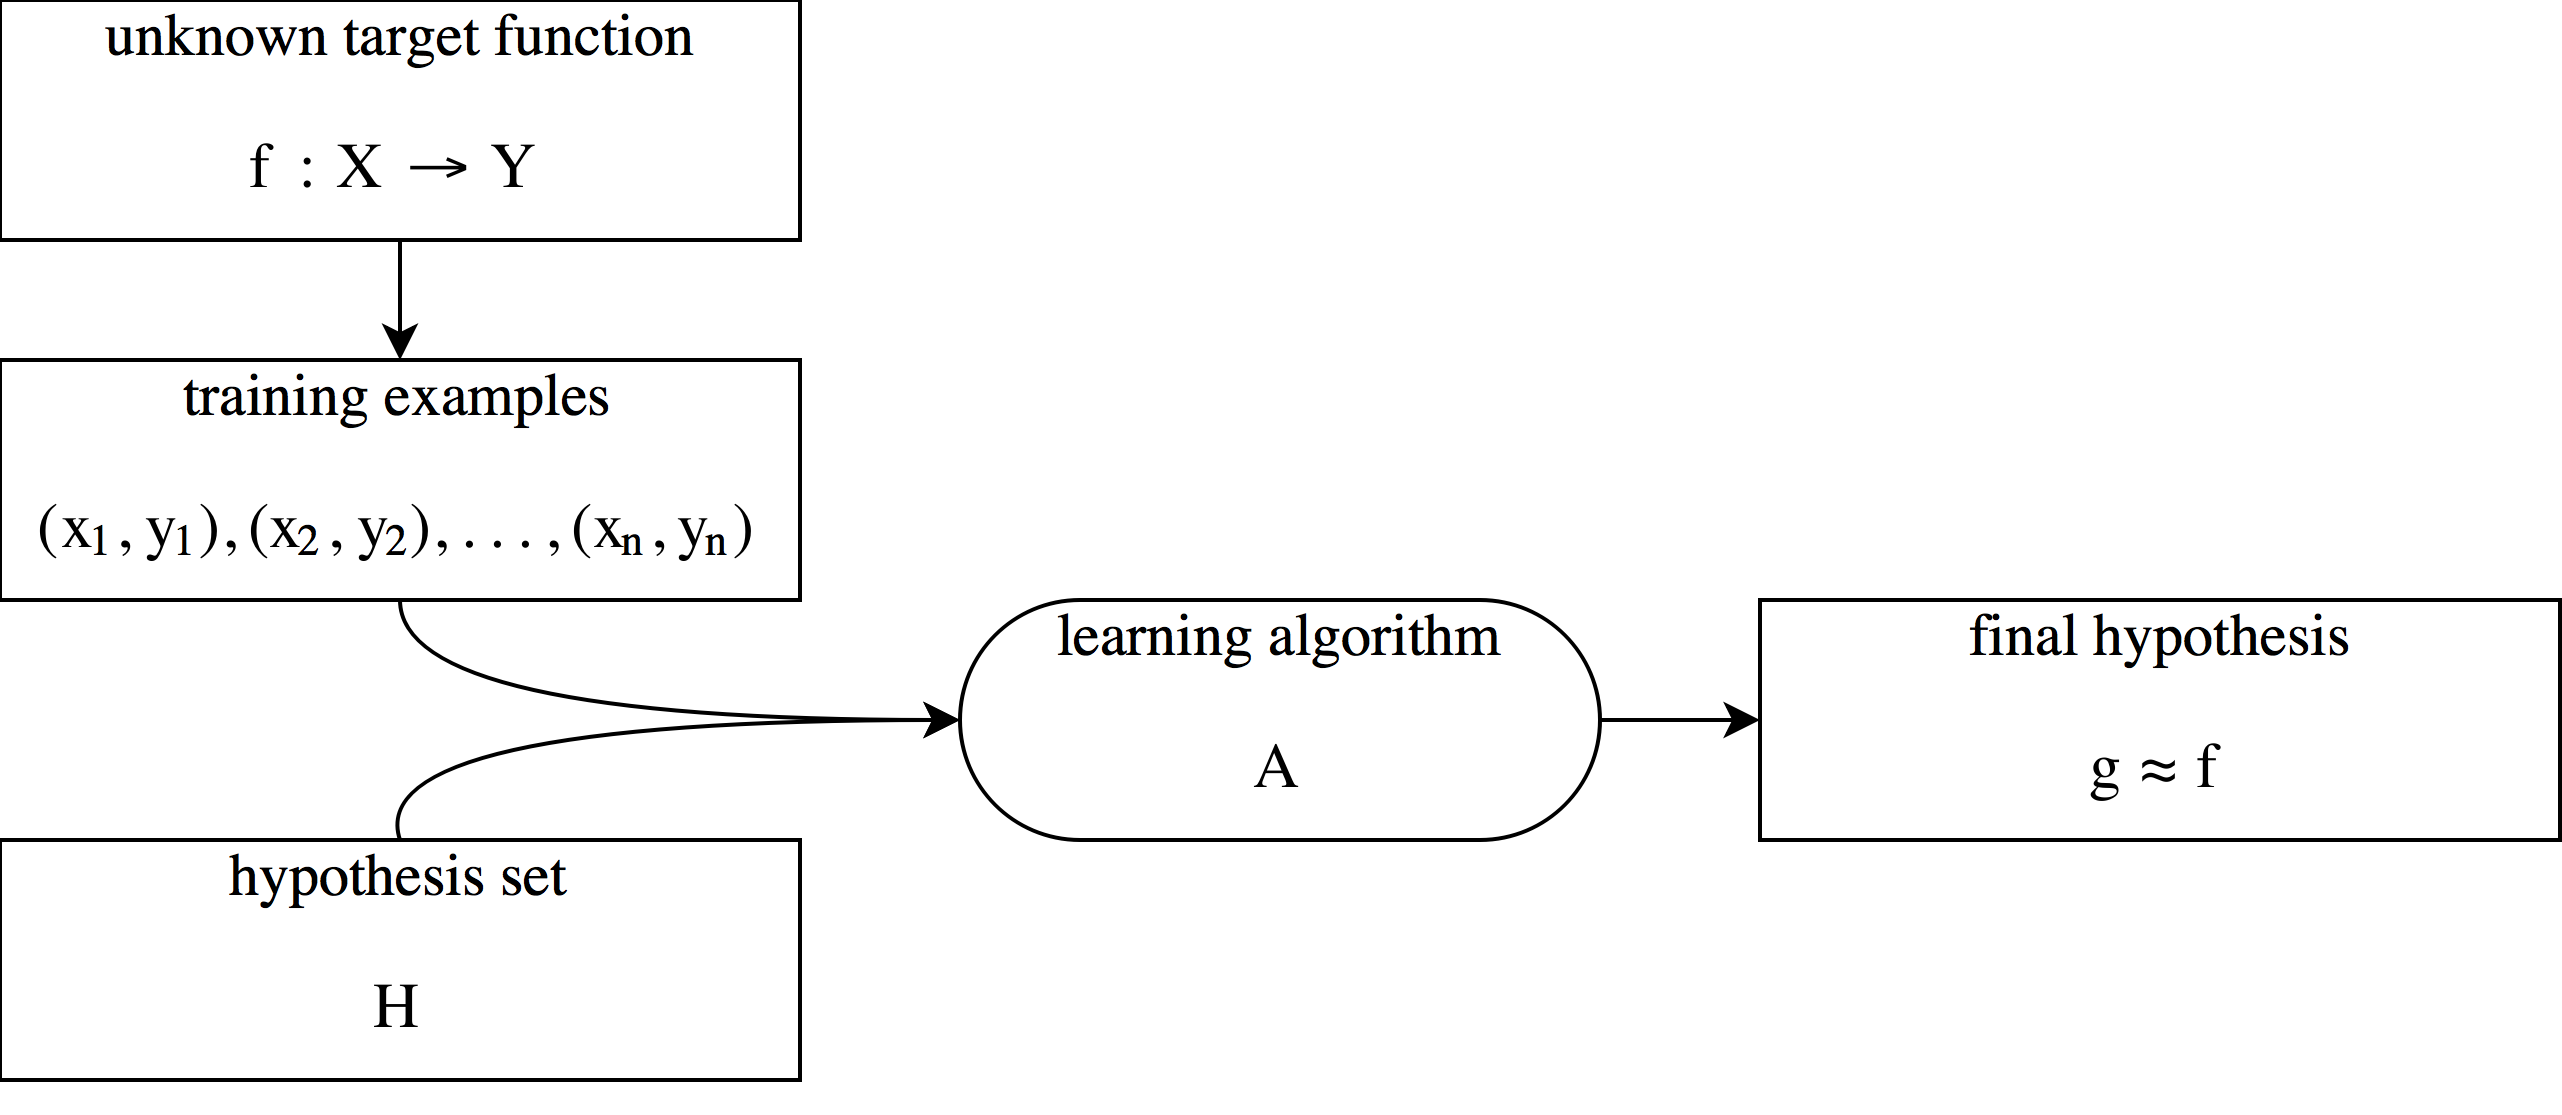
\includegraphics[width=\textwidth]{gfx/machine_learning.png}
\caption{The learning problem, adapted from \cite{abu2012learning}.}
\label{fig:learning_problem}
\end{figure}

\subsection{Supervised Learning}
The problem described above has some additional properties besides being a machine learning problem in general. Firstly, it falls in the category of supervised machine learning. Supervised learning is one of the three main learning paradigms of machine learning, together with reinforcement learning and unsupervised learning \cite{abu2012learning}. In the context of this thesis, the latter will be neglected as only supervised learning is used. It is characterized by the fact that the learning algorithm is provided with a set of inputs \textit{together} with the outputs, which could be viewed as a kind of teacher, or supervisor, explaining expected results to the learner. In the other cases, no such detailed feedback is provided to the learner. 

\subsection{Classification and Regression}
In addition to falling into the category of supervised learning, the problem is a classification problem. The nature of the prediction is to assign one of the three classes, also called labels, 'iris setosa', iris virginica' and 'iris versicolor' to a new plant. Formally, this means that the output space $Y$ of the target function consists of a finite set of labels $\lbrace y_1,\dots,y_n\rbrace$, so that each instance of the data set is associated with a label $y_i \in Y$, in this case $Y=\lbrace 'iris-setosa','iris virginica', 'iris versicolor' \rbrace $. 

Apart from classification, another important category of machine learning problems are regression problems. In the case of regression, the output space of the target function is no longer finite, but instead consist of real numbers. To reconsider the gardening example, the gardener could want to predict the height of a plant on the basis of the same features as used above. Likewise, they would have to observe a number of plants to gather feature values together with the expected target value, which instead of the species would then be the height of the plant in centimeters, that is $Y=\mathbb{R}$.

\subsection{Preference Learning}
% Why is label ranking relevant? -> for prediction based on preference
% Preference learning
Preference Learning is a relatively new subfield of machine learning \cite{DBLP:books/daglib/0025729}. It is dedicated to the problem of learning how to rank, the precise definition of what this encompasses being defined by the specific task one considers. Out of the three main tasks of preference learning, namely label ranking, instance ranking and object ranking, label ranking is the relevant one in the context of this thesis. But before going into the details of label ranking, it first has to be explained what is meant with a ranking in this context and how it is distinguished from the concept of an ordering, as it is easily confused.

\subsubsection{Ranking and Ordering}
To clarify the meaning of ranking and ordering, we return to the gardening example. After spending some time studying the different flowers, the gardener has realized he prefers certain iris species to others. He expresses his preference for a plant in a score, and labels all the plants in no particular order (see Fig. \ref{tab:ranking_vs_ordering}). An \textit{ordering} then is the result of simply ordering the labels in decreasing order of their respective score. It thus can also be given implicitly by just ordering the original classes, the flower names, as such being a permuation of the labels. A ranking, on the other hand, assigns a fixed position to each label; for instance the rank of 'iris virginica' will always be in the first position in the ranking, that is the number in that position denotes the \textit{rank} of the label, which is in turn defined as the label's position in the ordering. Therefore, the values in the example in Table \ref{tab:ranking_vs_ordering} result in the ranking $[2,3,1]$, whereas the ordering is $[3,1,2]$. It is notable that these can be the same, and are easily convertible. However, in the remainder of this thesis mostly the term ranking is used to identify both ranking and ordering interchangeably, especially as usually only the term 'ranking' is used.

\begin{table}[h]
\centering
	\begin{tabularx}{.8\textwidth}{>{\hsize=0.9\hsize}X | >{\hsize=.1\hsize}X >{\hsize=1.6\hsize\raggedleft\arraybackslash}X >{\hsize=1.6\hsize\raggedleft\arraybackslash}X >{\hsize=1.6\hsize\raggedleft\arraybackslash}X >{\raggedleft\arraybackslash} >{\hsize=.1\hsize}X}
		%\hline
		Species		& 	& \multicolumn{1}{>{\hsize=1.6\hsize\centering\arraybackslash}X}{iris virginica}	& \multicolumn{1}{>{\hsize=1.6\hsize\centering\arraybackslash}X}{iris versicolor}	& \multicolumn{1}{>{\hsize=1.6\hsize\centering\arraybackslash}X}{iris setosa}	& 	\\ \hline
		Label		& [ & 1,									& 2,										& 3 									& ] \\ 
		Score		& [ & 0.17,								& 0.12,									& 0.89 								& ] \\ 
		Ranking		& [ & 2,									& 3,										& 1 									& ] \\ 
		Ordering		& [ & 3,									& 1,										& 2 									& ] \\ 		
	\end{tabularx}
	\caption{Ranking and ordering in direct comparison.}
	\label{tab:ranking_vs_ordering}
\end{table}


\subsubsection{Label Ranking}
Similar to classification, in label ranking there is a finite set of labels $Y=\lbrace y_1,\dots,y_n \rbrace$, but it is not the output space. Instead, \citeauthor{DBLP:books/daglib/0025729} define the target function for label ranking as $f:X\rightarrow S_Y$ where the output space $S_Y$ contains all permutations over the set of labels $Y$ \cite{DBLP:books/daglib/0025729}. To come back to the topic of rankings and orderings, it becomes clear now that even though it is called label ranking, the labels are actually ordered. An example of label ranking could be, to stay in the domain of gardening, to learn the preferences of different gardeners towards iris plants. A label ranking data set used to learn this connection could, for example, map the favorite color and height of a gardener to a ranking of the three iris plants. 

\subsection{Meta Learning}
% Context is meta learning -> what does that mean and what are the consequence
The previous discussion of machine learning problems has conceptually been about the fitting of different machine learning algorithms to problems in the form of data sets. In the context of meta learning regarding machine learning, it is researched whether it is 'possible to learn about the learning process itself, and in particular that a system could learn to profit from previous experience to generate additional knowledge that can simplify the automatic selection of efficient models summarizing the data' \cite{brazdil2008metalearning}. That is, the original algorithm selection problem \cite{rice1976algorithm} is viewed as a learning problem itself that is to be tackled.

The approach of this thesis clearly falls under that category, as it is trying to learn whether a connection exists between properties of a data set, that is its meta features, and the performance values of certain classification algorithms, and how well it can be exploited by regression and preference models respectively, if it exists. The benefit from meta learning in the context of machine learning is that learning how properties of data sets influence the learning process of the classifiers could save much work; often, much work is put into the fitting of an algorithm to a specific data set, but it is not transferred to other problems that may be of the same nature.

\section{Evaluation}

After having discussed the preliminaries that the theoretical approach of this thesis is built upon, how a data set can be split into training and test data to estimate the performance of learning algorithms and the measures that will be used in the evaluation of the different ranking methods are briefly reviewed. These include means of comparing the predicted rankings with actual rankings as well as a statistic that reveals whether an advantage regarding one measure can be viewed as significant.

\subsection{Estimation Procedures}

To find out how well a classifier performs, it first needs to be decided which measure to consider. There are a few possibilities for this, however in this thesis the term performance measure refers to the predictive accuracy of a classifier, that is the percentage of classes that a classifier correctly identified in a given data set. But since using the whole data set to train a classifier, that is build a model, would skew the analysis - the classifier has already 'seen' these examples - a method for dividing data sets into train and test sets is needed. 

A popular approach is using a stratified split, for example splitting the data into 70\% training and 30\% test data, with the important aspect that both subsets have equal (or at least very similar) ratios of classes [Reference Missing]. The learning algorithm is then trained with one part of the data (usually the larger), and its performance tested on the other. To get more stable results, often the process is repeated: The data is divided in k folds, k times, the learning algorithm is trained on k-1 folds, and tested on the left out subset. Results are averaged. This process is then called k-fold (stratified) cross-validation [Reference Missing]. A variant of this is Monte Carlo cross-validation, where after each time the algorithm has been trained and evaluated, a new split is randomly computed [Reference Missing]. This especially causes the fact that the number of folds does not dictate the ratio of the split; one could for example have 5-folds Monte Carlo cross-validation with a 70\%/30\% train/test split.

An alternative to using a stratified split is using a method called leave-one-out. This method essentially is, for a data set with n instances, n-fold cross-validation (not stratified, naturally). This means that the algorithm is trained on n-1 instances and evaluated on the instance that has been left out.

\subsection{Kendall Rank Correlation Coefficient}
% We need to evaluate the ranker quality somehow, ranker predicts rank, so need a 
To evaluate the quality of the prediction that a ranker will make, a statistic is needed to compare a predicted ranking with the correct ranking. For this, the Kendall Rank Correlation Coefficient will be used here, as it expresses the similarity of two rankings.

% Definition of Kendall
The Kendall Rank Correlation Coefficient, also known as Kendall's tau, is a measure of association between two rankings of the same items \cite{kendall1938new}. For two independent variables $X$ and $Y$ and observations of values $(x_1,x_2,...,x_m)$ for $X$ and $(y_1,y_2,...,y_n)$ for $Y$ with unique $x_i$ and $y_i$ respectively, the coefficient is based on comparing pairs of observations. If for two pairs $(x_i,y_i)$ and $(x_j,y_j)$ both $x_i < x_j$ and $y_i < y_j$ (or the opposite) holds, they are viewed as concordant. If $x_i < x_j$ but $y_i > y_j$ (or the opposite), they are viewed as discordant. Other cases are not considered. The simplest version of the statistic, called $T_A$ is then defined as 

$$T_A = \frac{n_c - n_d}{n_0},$$
with \\
$n_c$, the number of concordant pairs, \\
$n_d$, the number of discordant pairs, and \\
$n_0 = n * (n - 1) / 2$.

To account for ties in the rankings, a second statistic, $T_B$ is defined as

$$T_B = \frac{n_c - n_d}{\sqrt{(n_0 - n_1 )(n_0 - n_2 )}},$$
with \\
$n_c$, $n_d$, $n_0$ as above, \\
$n_1=\sum_i{t_i(t_i-1)/2}$, \\
$n_1=\sum_j{t_j(t_j-1)/2}$, \\
$t_i,$ the number of ties observed for X in the ith position of the ranking \\
$u_j,$ the number of ties observed for Y in the ith position of the ranking 

Thus, the value of the tau (for both versions) lies in the interval $[-1,1]$, with 1 indicating a perfect agreement of rankings, -1 perfect disagreement, and 0 corresponding to no correlation. A high value is therefore desirable in this context, as it indicates that the prediction of the ranker agrees with the actual ranking of algorithms.

\subsection{Loss}
While the Kendall rank correlation coefficient is an indication as to what degree a predicted ranking agrees with the correct ranking of classifiers for a certain data set, it does not convey the difference in performance experienced by the user when choosing the first of the recommended algorithms. This difference can be expressed in a measure called loss \cite{DBLP:conf/mldm/LeiteBV12}, which is defined as the difference of the performance of the actual best algorithm and the actual performance of the first recommended algorithm. 

Additionally, the ranker recommends a ranking instead of a single algorithm in order to allow a user (or automated tool) to test a few of the top-ranked algorithms, which therefore also needs to be taken into account when thinking about loss. This is done here by computing a measure called best three loss, which denotes the loss resulting in the selection of the best of the first three recommended classifiers in comparison to the actual best-performing classifier in the considered set of classifiers. 

\subsection{Mann-Whitney U Test}
The measures previously presented can indicate if one of the ranking alternatives is superior to another regarding that measure, but one cannot conclude from those results alone whether this advantage is significant. The question here is whether the null-hypothesis that two distributions belong to the same population can be rejected. This can be determined with the help of the Mann-Whitney U, a non-parametric hypthesis test \cite{mann1947test}. The Mann-Whitney U is computed by, for two distributions one wants to analyze, counting how many times each value from one distribution is lower than another value from the other distribution. If the U is very high (or low, depending on the hypothesis), the null hypothesis can be rejected. Whether this significance level is reached is expressed by the p-value: for a p-value below 0.05, the null hypothesis can be rejected. Therefore, if two distributions, for example regarding the loss values of two ranking approaches, suggest that one is superior to the other, and the p-value for the Mann-Whitney U is <= 0.05, this suggests that the difference is statistically significant.
